\section{Hauptteil}
\subsection{Meilensteine}
Zu Beginn des Projekts haben wir Meilensteine festgelegt, die zeitliche Ziele enthalten, die zu einem bestimmten Zeitpunkt erreicht werden müssen.
Diese Ziele können vielfältig sein, von einfacheren Aufgaben wie der Recherche von Frameworks für Linux, Windows und Android bis hin zu komplexeren und vielfältigeren Zielen wie der Implementierung von Nachrichtenversand und Anrufen.
Im ersten Anhang finden Sie meine vollständige Meilensteinsetzung. \\\\
Gemäss meiner Meilensteinsetzung war meine erste Aufgabe, Go im Hinblick auf
GUI-Entwicklung zu erlernen. Für das Windows-Framework habe ich mich für Wails \cite{wails} entschieden, während ich mich für Linux für GTK entschieden habe.
Ursprünglich wollte ich QT \cite{qt} für Linux nutzen, aber es konnte nicht richtig kompiliert werden, da das von mir gewünschte Framework veraltet war. Deshalb habe ich mich für Gogtk3 \cite{gogtk3} entschieden.
\subsection{Funktionen, Elementtypen und Variabeln in Go}
\subsubsection{Eine Einführung in die verschiedenen Variablentypen in Go}
In Go gibt es vielfältige Variabletypen, darunter Strings, Integers und Unsigned Integers. In diesem Abschnitt werde ich versuchen, diese auf möglichst einfache und kompakte Weise zu erläutern. Beginnen wir mit Strings: Strings in Go können jeden beliebigen Wert aufnehmen, es muss nicht zwangsläufig UTF-8 sein, es könnte jeglicher Wert sein.\\\\
Ein Integer hingegen kann nur Zahlenwerte innerhalb des definierten Bereichs aufnehmen. Hierbei muss berücksichtigt werden, ob man einen int8 (Byte), int16, int32 oder int64 definiert, da jeder dieser Typen einen anderen Wertebereich besitzt. Ein int8 reicht von -128 bis 127, ein int16 von -32768 bis 32767, ein int32 von -2147483648 bis 2147483647 und ein int64 von -9223372036854775808 bis 9223372036854775807.\\\\
Darüber hinaus gibt es noch Unsigned Integers, die nur Werte grösser oder gleich Null speichern können, und deren Wertebereich jeweils von 0 bis zur Summe aus der negativen und der positiven Zahl der entsprechenden Integer-Typen reicht.\\\\
Es gibt auch noch Gleitkommazahlen, Slices und viele weitere Typen. Für ausführlichere Informationen verweisse ich euch auf die Golang Spezifikationen\footnote{Golang Spezifikationen: https://go.dev/ref/spec}.
\subsubsection{Definition und Verwendung von Variabeln in Go}
Es existieren zahlreiche Methoden zur Definition von Variablen in Go. Unter anderem kann man eine Variable vorab deklarieren, wie nachstehend dargestellt:
\begin{lstlisting}
var name string
\end{lstlisting}
Dieser Codeausschnitt deklariert eine Variable vom Typ String mit dem Namen "name". Für die Nutzung in einem Programm könnte man sie wie folgt einsetzen:
\begin{lstlisting}
name = fmt.Sprintf("Cedric")
\end{lstlisting}
Allerdings habe ich diesen Ansatz nur sporadisch genutzt, da man hierfür zunächst den Typ festlegen muss. Deshalb habe ich meistens die dynamische Variablendeklaration verwendet, die eine Variable vom Typ "string" mit dem Namen "name" wie folgt definiert:
\begin{lstlisting}
name := fmt.Sprintf("Cedric")
\end{lstlisting}
\subsubsection{Definition und Verwendung von Funktionen in Go}
Zur Definition einer Funktion in Go benötigt man das Schlüsselwort "func", gefolgt von dem Namen der Funktion. Für eine Funktion namens "helloWorld" könnte man das wie folgt formulieren:
\begin{lstlisting}
func helloWorld() {}
\end{lstlisting}
Die runden Klammern stehen für die Parameterliste und die geschweiften Klammern für den Funktionskörper. Um einen Parameter des Typs String mit dem Namen "name" hinzuzufügen, der mit "Hallo" zusammengefügt und zurückgegeben wird, wäre der entsprechende Code folgender:
\begin{lstlisting}
func helloWorld(name string) {
  fmt.Printf("Hallo, %s", name)
}
\end{lstlisting}
Dies ist eine Funktion, die lediglich den Namen auf der Standardausgabe ausgibt. Es ist jedoch auch möglich, dass Funktionen Werte zurückgeben. In diesem Fall muss der Rückgabewert in der Funktionsdeklaration angegeben und vorab mit dem Schlüsselwort "return" geschrieben werden, was etwa so aussehen könnte:
\begin{lstlisting}
func helloWorld(name string) string {
  return fmt.Sprintf("Hallo, %s", name)
}
\end{lstlisting}
\subsection{Die ersten Schritte}
Wie bereits erwähnt, bestand meine erste Aufgabe darin, GUI-Frameworks zu recherchieren. Meine zweite Aufgabe war die Erstellung einer einfachen Anwendung mit einem Texteingabefeld.
\begin{figure}[h]
\centering
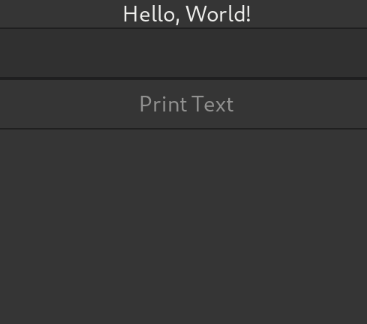
\includegraphics[width=0.5\textwidth]{txt/pictures/simple_window.png}
\caption{Ein GTK-Fenster, das ein Textfeld beinhaltet.}
\label{fig:example}
\end{figure}
\\
Da dies mein erstes Programm war, wollte ich es nicht zu kompliziert gestalten. Das Programm gibt den Text aus dem Eingabefeld auf stdout aus.
\subsection{GUI entscheid}
\subsubsection{Wails als GUI Framework}
Eine gewisse Zeit lang präferierte ich das GUI-Entwicklungswerkzeug namens Wails, konnte mich jedoch nicht endgültig dafür entscheiden. Dennoch konnte ich meine bestehende Gtk-Anwendung innerhalb von lediglich zwei Stunden komplett umgestalten, ein Prozess, der in Gtk ganze drei Tage beansprucht hätte. Ein zusätzlicher Nutzen von Wails besteht darin, dass man JavaScript und HTML für die Fenstergestaltung einsetzen kann. Darüber hinaus offeriert Wails eine geschätzte Funktion mit der Bezeichnung 'Automatische Neukompilierungen' \cite{wailsAutoRebuild}, welche es mir ermöglicht, Code-Modifikationen vorzunehmen und das Programm automatisch zu aktualisieren. Von Linux aus ist es ferner einfacher, für Windows und MacOSX zu kompilieren. In einem späteren Abschnitt werde ich detaillierter auf die Gründe eingehen, warum ich von Wails zu Fyne gewechselt bin.
\subsubsection{Fyne als GUI-Framework}
Letztendlich habe ich mich für Fyne \cite{fyne-web} entschieden, das ich nunmehr auch finanziell unterstütze (siehe den Zweiten Anhang für die Quittung), da es mich aufgrund seiner herausragenden Eigenschaften überzeugt hat. Indem ich nun ein Framework verwende, das meinen Code nicht in eine andere Programmiersprache kompilieren muss, steht mir die Möglichkeit offen, sämtliche Go-Funktionen sowie Bibliotheken zu nutzen. Dies eröffnet mir den Weg, komplexere Anwendungen zu erstellen. Darüber hinaus ermöglicht mir Fyne, nicht nur für Windows/Linux, wie bei Wails, sondern auch für Android zu kompilieren. Dies hat den Vorteil, dass ich lediglich eine Codebasis pflegen muss, anstatt zwei separate zu schreiben.
\subsection{Erstes Projekt}
Mein erstes Projekt mit dem Wails-Framework war eine einfache plattformübergreifende Wetter-App unter Verwendung der OpenWeatherAPI. Die App ist nur für die Stadt Winterthur verfügbar, da es schwierig ist, den GPS-Standort in Go zu ermitteln, und zu dem ich dies auch nicht in meinem Projekt brauche, da dass die Privatsphäre minimiert.
\subsection{Verschlüsselungs-Stack}
Mein geplanter Verschlüsselungs-Stack soll die folgenden Algorithmen nutzen: \hyperref[glo:blake]{\(blake2b\_512^{[d]}\)}, \hyperref[glo:ecc]{\(ECC^{[e]}\)}, \hyperref[glo:aes]{\(AES^{[f]}\)} und \hyperref[glo:crystal-dilithium]{\(CRYSTAL-Dilithium^{[g]}\)}. 
\\
Ich habe mich für einen derart komplexen Verschlüsselungs-Stack entschieden, da mein Messenger höchsten Wert auf Sicherheit und Privatsphäre legt. Deshalb habe ich einen Algorithmus integriert, der auch gegenüber Angriffen durch Quantencomputer noch zuverlässig schützt. Denn ich bin der Überzeugung, dass es von essentieller Bedeutung ist, auch vor zukünftigen Angriffsmethoden geschützt zu sein. In meinen Augen ist die Zukunft bereits jetzt mit Quantencomputern angebrochen.
\\
Ich habe mich für den CRYSTAL-Dilithium-Algorithmus entschieden, da er von NIST empfohlen wird. \cite{nist-recomedation}
\subsubsection{Erstellung des Entschlüsselungs Modules}
Mein Ziel war es, ein möglichst modulares Entschlüsselungsmodul zu erstellen. Aus diesem Grund plante ich, das Modul mit einer Vielzahl von Funktionen zu schreiben, um es mir zu ermöglichen, mein Verschlüsselungsmodul in einem anderen Go-Paket zu importieren und zu nutzen.
\subsubsection{Key Pair Erstellung}
Ich muss zunächst zwei verschiedene Key-Paare für ECC und Dilithium generieren, unter Verwendung der nachfolgenden Funktionen:
\begin{lstlisting}[language=Go]
func GenerateECCKeyPair(curve elliptic.Curve) (*ecdsa.PrivateKey,
                                               *ecdsa.PublicKey, 
                                               error) {
	privateKey, err := ecdsa.GenerateKey(curve, rand.Reader)
	if err != nil {
		return nil, nil, err
	}

	publicKey := &privateKey.PublicKey

	return privateKey, publicKey, nil
}

func GenerateDilithiumKeyPair(modeName string) (dilithium.PublicKey,
                                                dilithium.PrivateKey, 
                                                error) {
	mode := dilithium.ModeByName(modeName)
	if mode == nil {
		return nil, nil, fmt.Errorf("mode not supported")
	}

	publicKey, privateKey, err := mode.GenerateKey(rand.Reader)
	if err != nil {
		return nil, 
                       nil,
                       fmt.Errorf("error generating key pair: %v", err)
	}

	return publicKey, privateKey, nil
}
\end{lstlisting}
Dieser Code erzeugt zwei Key Pairs und gibt sie mir zurück, damit ich sie in einer Variablen speichern und später zur Signierung von Nachrichten verwenden kann. Wie aus dem Code ersichtlich, geben beide Funktionen jeweils drei Werte zurück, nämlich den Private- bzw. den PublickKey und einen Fehler, falls ein solcher auftreten würde.
\subsubsection{Unterschrift}
Die folgenden Funktionen dienen der Signatur von Nachrichten, um sicherzustellen, dass diese tatsächlich von der Person gesendet wurden, von der man annimmt, dass sie sie gesendet hat. Es handelt sich dabei um zwei Funktionen:
\begin{lstlisting}[language=Go]
func SignEcc(privateKey *ecdsa.PrivateKey, messageHash []byte) ([]byte,
                                                                error) {
	r, s, err := ecdsa.Sign(rand.Reader, privateKey, messageHash)
	if err != nil {
		return nil, err
	}

	curveBits := privateKey.PublicKey.Curve.Params().BitSize
	keyBytes := (curveBits + 7) / 8

	signature := make([]byte, keyBytes*2)
	rBytes := r.Bytes()
	sBytes := s.Bytes()

	copy(signature[keyBytes-len(rBytes):], rBytes)
	copy(signature[keyBytes*2-len(sBytes):], sBytes)

	return signature, nil
}

func SignDilithium(
	privateKey dilithium.PrivateKey,
	msg []byte,
	modeName string,
) ([]byte, int, error) {
	mode := dilithium.ModeByName(modeName)
	if mode == nil {
		return nil, -1, fmt.Errorf("mode not supported")
	}

	signatureSize := mode.SignatureSize()

	return mode.Sign(privateKey, msg), signatureSize, nil
}
\end{lstlisting}
Bei den beiden zuvor genannten Funktionen besteht ein erheblicher Unterschied, insbesondere bei der SignEcc-Funktion. Hierbei unterzeichne ich nicht direkt die Nachricht selbst, sondern den Hashwert, der mir von der Funktion, die auf dem Blake2b-Algorithmus basiert, ausgegeben wird. Die Nachfolgende Funktion ist meine Implementation davon:
\begin{lstlisting}
func CalculateHash(message []byte) []byte {
	hash, err := blake2b.New256(nil)
	if err != nil {
		fmt.Printf("Error creating hash: %v\n", err)  
		return nil
	}
	hash.Write(message)
	return hash.Sum(nil)
}
\end{lstlisting}
\subsection{Erstellung einer Sidebar mit Gravatars: Erfahrungen und Ergebnisse}
Ich habe ein Template für die Sidebar erstellt, welche mit Gravatars gefüllt ist, um zu sehen, ob die Sidebar mit Profilbildern gut aussieht. Die Arbeit an der Sidebar war komplex, da ich zuvor noch keine Erfahrung mit der Erstellung von Sidebar-Elementen mittels \hyperref[glo:html1]{\(HTML^{[a]}\)}, \hyperref[glo:css]{\(CSS^{[b]}\)}, \hyperref[glo:js]{\(JS^{[c]}\)} und GO hatte. Meines Erachtens ist das Ergebnis jedoch sehr gelungen.
\subsection{Design}
\subsubsection{Tool}
Ich habe mir verschiedene Design-Umgebungen im Internet angesehen und bin auf zwei Vergleichslisten \cite{figma-entschied-1}\cite{figma-entschied-2} gestossen, auf denen 17 bzw. 6 Design-Tools miteinander verglichen wurden. Nachdem ich festgestellt habe, dass Figma auf beiden Listen aufgeführt ist, habe ich mich für diese Design-Plattform entschieden.
Ich habe herausgefunden, dass Figma auch auf Linux installiert werden kann, wie ich auf der folgenden Website \cite{figma-linux} erfahren habe. Allerdings muss ich gestehen, dass es sich bei Figma um proprietäre Software handelt, was bedauerlich ist.
\subsubsection{Arbeit}
Ich habe mein GUI zunächst mit dem spezialisierten Design-Tool namens Figma erstellt. Zuvor hatte ich mir das Tool noch nie angesehen, sodass ich es von Grund auf lernen musste. Figma ist äusserst vielseitig und bietet viele nützliche Tools, die beim Designen helfen.
Um das Tool kennenzulernen, habe ich ein Demo-Interface erstellt, das auf einem Tutorial \cite{figma-tutorial} basierte. Das Tutorial ermöglichte es mir, die meisten Funktionen des Tools innerhalb eines Morgens zu erlernen und zu nutzen.
\subsection{Server}
\subsubsection{Warum ich lange Zeit mit WebSockets gearbeitet habe}
Ich habe mich für einen Server entschieden, der WebSockets verwendet, aus einer Vielzahl von Gründen.\\
Einige davon sind:  \cite{fette2011websocket}\cite{gupta2017websockets}
            \begin{enumerate}
                \item Nahtlose Integration mit Web-Technologien: Da WebSockets auf dem Web-Standard aufbauen, gestaltet sich ihre Integration in Webanwendungen mühelos und gewährleistet eine konsistente Kommunikation über verschiedene Plattformen hinweg.
                \item Bidirektionale Vollduplex-Kommunikation: Im Unterschied zu HTTP ermöglichen WebSockets eine bidirektionale, vollduplexe Kommunikation zwischen Client und Server. Dies befähigt den Messenger-Dienst zur Echtzeitdatenübertragung und verbessert die Interaktivität zwischen Nutzern.
                \item Geringerer Overhead: Im Gegensatz zu HTTP-Polling oder Long-Polling-Techniken benötigen WebSockets nach dem Handshake keine zusätzlichen HTTP-Header für jede Nachricht und verbrauchen somit weniger Bandbreite.
                \item Verbindungszustand: Anders als HTTP, das zustandslos ist, bewahrt WebSockets einen Verbindungszustand bei, wodurch die Kommunikation effizienter wird und die Latenzzeit reduziert wird.
                \item Überwindung von Firewalls und Proxies: WebSockets können ohne Schwierigkeiten über Firewalls und Proxies kommunizieren, da sie auf dem HTTP-Upgrade-Mechanismus aufbauen, was die Einrichtung und Verwendung von Messenger-Diensten erleichtert.
                \item Multiplexing und Priorisierung: WebSockets unterstützen das Multiplexing von mehreren Nachrichtenströmen über eine einzige Verbindung, wodurch die Netzwerkauslastung verringert und die Kommunikationsleistung verbessert wird.
                \item Standardisierung  \cite{8757486}: WebSockets sind ein weithin verbreiteter und standardisierter Kommunikationsmechanismus, der die Implementierung und Integration erleichtert.
                \item Skalierbarkeit: Durch die Nutzung der WebSockets-Technologie kann mein Messenger-Dienst einfach und effizient skaliert werden, um eine grosse Anzahl gleichzeitiger Benutzer zu unterstützen.
                \item Echtzeit-Synchronisation: Dank WebSockets kann eine Echtzeit-Synchronisation realisiert werden, die den Nutzern die kontinuierliche Nutzung der Applikation ohne das ständige Neuladen ermöglicht, um eine neue Nachricht zu erhalten.
            \end{enumerate}
Eine Alternative zum WebSocket stellt das TCP/IP-Modell dar. Jedoch geht mit dessen Verwendung das Risiko von Verbindungsabbrüchen und Paketverlusten einher. Im Gegensatz dazu erfordern WebSockets geringere Ressourcen und sind aufgrund ihrer Einzelverbindung einfacher umzusetzen. Trotzdem können beide Protokolle in bestimmten Anwendungsfällen nützlich sein und ihre Eignung hängt von den spezifischen Anforderungen der jeweiligen Anwendung ab.
\subsubsection{Warum ich mich letztendlich für WebRTC anstelle von Websockets entschieden habe.}
WebRTC \cite{webrtc-website} bietet nicht nur zahlreiche Funktionen wie beispielsweise Voice- und Videotelefonie sowie das Übertragen von Dateien und Nachrichten über die WebRTC Data Channels, sondern verfügt auch über eine integrierte Verschlüsselungs- \cite{rfc8829} und Authentifizierungsmöglichkeit. Darüber hinaus ist WebRTC auch P2P, was bedeutet, dass keine Server erforderlich sind und die Nachrichten nur auf den Handys der Mitglieder gespeichert werden. \\
Für die Voice- und Videotelefonie können Sie sich bei Matrix umschauen, da sie auch WebRTC für diese Funktionen nutzen. \cite{matrix-website}\\
Für den Nachrichtenaspekt können Sie sich hier \cite{webrtc-msg} umschauen. Hier ist eine beispielhafte Implementierung, um Nachrichten über den Data Channel zu übertragen, wodurch mir bewusst ist, dass es funktionieren kann.
\subsection{Entwicklung der Server Software}
Für mein Server-Modell habe ich zunächst einen simplen Chatroom erstellt, in dem bis zu 16 Personen gleichzeitig teilnehmen können. Da ein Chatroom jedoch lediglich eine Chat-Funktion bereitstellt, musste ich den Code modifizieren, um für jeden Chat einen eigenen privaten Chatraum zu erstellen. Des Weiteren hatte mein einfacher Chatraum keine Verschlüsselung, die ich hinzufügen musste. Dies war jedoch kein Problem, da ich meinen Verschlüsselungs-Stack bereits zwei Wochen zuvor äusserst modular geschrieben hatte, was mir in diesem Fall sehr zugutekam.
\subsubsection{WebRTC messaging Implemntieren}
Um die Implementierung von WebRTC-Messaging zu realisieren, habe ich den in JavaScript verfassten Quellcode \cite{webrtc-messegaing-example-js} in Go-Code umgewandelt, der von meinem Programm interpretiert werden kann.
\subsection{WebRTC vs. Websocket Code}
Die Disparität zwischen Websockets und WebRTC erwies sich für mich als erheblich, da ich bis zu diesem Zeitpunkt noch keine Erfahrungen mit WebRTC gesammelt hatte. Im Nachfolgenden beabsichtige ich, die Unterschiede zu verdeutlichen, beginnend mit der Darstellung meiner ursprünglichen Implementierung von Websockets, gefolgt von meiner Umsetzung von WebRTC, für die ich letztlich optierte.
\subsubsection{Websockets}
Die Implementierung von Websockets stellte sich für mich als unerfahrenen Entwickler von Netzwerkanwendungen zunächst als Herausforderung dar, da mir die notwendige Erfahrung fehlte. Jedoch erleichterte mir die Websocket-Bibliothek \cite{websocket-lib-nhooyr} die Aufgabe, einen Gruppen-Chat-Raum zu erstellen, obwohl mein eigentlicher Ziel eher in der Gestaltung eines P2P-Messengers lag. Darüber hinaus ist die genannte Websocket-Implementierung nicht die am weitesten verbreitete; vielmehr wird die Implementierung hier \cite{websocket-lib-gorrila} am häufigsten genutzt. Allerdings halte ich das für ein Problem, da sie am 09.12.2023 archiviert wurde, weshalb ich mich letztlich dagegen entschied, diese Bibliothek zu verwenden.
\subsection{Backend-as-a-Service (BaaS): Technologieauswahl und Implementierungsstrategien}
\subsubsection{Umstellung auf die Pusher-Plattform: Beweggründe und Vorteile}
Ich habe in der Vergangenheit eine beträchtliche Zeitspanne damit verbracht, mich mit der Konzeption einer proprietären Server-Plattform zu befassen. Allerdings bin ich durch eine steigende Disparität zwischen meinem zeitlichen Aufwand und den zur Verfügung stehenden Ressourcen konfrontiert worden, was mich dazu veranlasste, meine Prioritäten neu zu bewerten. \\\\
Letztendlich habe ich dazu optiert, eine bereits vorentwickelte Plattform zu adaptieren, die es ermöglicht, Änderungen an meinen Daten durch einfache API-Interaktionen vorzunehmen. Diese Option präsentiert sich als eine signifikante Effizienzsteigerung gegenüber dem vorigen Ansatz, indem sie die administrative Belastung erheblich reduziert und gleichzeitig eine robuste Funktionalität gewährleistet. \\\\
Die Plattform, für die ich mich entschieden habe, hört auf den Namen 'Pusher'. Pusher stellt eine optimalisierte Lösung dar, die eine nahtlose Integration und ein effektives Datenmanagement ermöglicht, was meine Bedürfnisse und Erwartungen in diesem Kontext perfekt erfüllt.
\subsubsection{Die Wahl von Supabase für den Nutzerauthentifizierungsprozess: Flexibilität, Skalierbarkeit und Datensicherheit}
Zur Implementierung des Nutzerauthentifizierungsprozesses erschien mir der Einsatz einer Open-Source-Alternative zu Google Firebase, allgemein als Supabase bekannt, als überaus adäquat. Diese Entscheidung fusst auf einer Vielzahl von Faktoren, insbesondere jedoch auf der beeindruckenden Flexibilität und Skalierbarkeit von Supabase, gerade im Hinblick auf die Übertragungskapazitäten in der gebührenfreien Ausführung.\\\\
Supabase brilliert durch seine Fertigkeit, substantielle Datenmengen zu transferieren, wodurch meine Prämissen bezüglich der Datenverwaltung in beachtlichem Masse erfüllt werden. Ferner offeriert es eine robuste und sichere Plattform für die Nutzerauthentifizierung, die von essentieller Bedeutung für jedwedes zeitgenössische digitale Produkt ist.\\\\
Es entspricht meinem primären Vorhaben, insbesondere im Kontext der Nutzerauthentifizierung auf Supabase zu vertrauen. Es verspricht eine nahtlose und intuitive Benutzererfahrung, die sowohl dem Endnutzer als auch dem Entwickler zugutekommt. Mit der Verwendung von Supabase bin ich in der Lage, die Authentifizierung meiner Nutzer sicher und effizient zu gewährleisten, wobei ein besonderes Augenmerk auf Datensicherheit und Benutzerfreundlichkeit liegt.
\subsection{Nutzerauthentifizierung implementation in JS, für SupaBase}
Zur Authentifizierung eines Anwenders mittels JS für SupaBase erweist es sich als unabdingbar, zuerst einen SupaBase-Client zu konstituieren. Die Verwirklichung dieser Prämisse lässt sich dem untenstehenden Quellcode entnehmen, der als tragendes Gerüst für den fortlaufenden JS-Code in dieser Sektion dient. Dieser JS-Code wurde von hier \cite{supabase-js-client-new-addititional-parameters} adaptiert, sodass er die API-Schlüssel von meinem unmittelbar darauf folgenden Go-Code extrahieren kann:
\begin{lstlisting}
import { RetrieveEnvValues } from "../wailsjs/go/main/App.js";
import { createClient } from "https://cdn.jsdelivr.net/npm/@supabase/supabase-js@2";

const options = {
  db: {
    schema: "public",
  },
  auth: {
    autoRefreshToken: true,
    persistSession: true,
    detectSessionInUrl: true,
  },
};

let supabaseKey;
let supabaseUrl;
let supabase;

RetrieveEnvValues().then((env) => {
  console.log(`Env: ${env}`);
  supabaseKey = env.supaBaseApiKey;
  supabaseUrl = env.supaBaseUrl;
  console.info(`Supabase Key: ${supabaseKey}`);
  console.info(`Supabase URL: ${supabaseUrl}`);
  console.info(`Supabase options: ${JSON.stringify(options)}`);
  supabase = createClient(supabaseUrl, supabaseKey, options);
});
\end{lstlisting}
Der im Anschluss präsentierte Go-Code extrahiert die Daten für die in Gebrauch genommenen API-Schlüssel aus einer Datei namens .env. Sie werden in die Struktur mit der Bezeichnung Config eingegliedert und nach Abschluss dieser Operation zurückgegeben:
\begin{lstlisting}
import 	"github.com/joho/godotenv"

type Config struct {
	AppId          string `json:"appId"`
	AppSecret      string `json:"appSecret"`
	AppKey         string `json:"appKey"`
	ClusterId      string `json:"clusterId"`
	SupaBaseApiKey string `json:"supaBaseApiKey"`
	SupaBaseUrl    string `json:"supaBaseUrl"`
}

func (a *App) RetrieveEnvValues() Config {
	m := &utils.MessengerUtils{
		Verbose: a.verbose,
	}
	m.PrintInfo("Loading .env file")
	err := godotenv.Load()
	if err != nil {
		utils.PrintError("Error loading .env file", err)
		return Config{}
	}
	a.config.AppId = os.Getenv("APP_ID")
	a.config.AppSecret = os.Getenv("SECRET")
	a.config.AppKey = os.Getenv("KEY")
	a.config.ClusterId = os.Getenv("CLUSTER")
	a.config.SupaBaseApiKey = os.Getenv("SUPABASE_API_KEY")
	a.config.SupaBaseUrl = os.Getenv("SUPABASE_URL")
	m.PrintInfo("The app_id is: "+a.config.AppId,
		"The app_secret is: "+a.config.AppSecret,
		"The app_key is: "+a.config.AppKey,
		"The cluster_id is: "+a.config.ClusterId)
	return a.config
}
\end{lstlisting}
Eine exemplarische .env-Datei, abgestimmt auf den vorausgegangenen Go-Code, könnte folgendermassen konstruiert sein. Es sei jedoch angemerkt, dass die im nachstehenden Beispiel genannten Daten keine validen Anmeldedaten darstellen, sie entsprechen lediglich dem korrekten Format:
\begin{lstlisting}
APP_ID="7911732"
SECRET="e78d5c1e258ae511ff79"
KEY="f589k16321h0db19812g"
CLUSTER="eu"
SUPABASE_API_KEY="eyJhbGciOiJIUzI1NiIsInR5cCI6IkpXVCJ9.
eyJ1c2VyX2lkIjoxMjMsInJvbGUiOiJ1c2VyIn0.
35p_Ah1xy2v1NBIENeSECXVPVm5ydsFhoGcVqQBkRMU"
SUPABASE_URL="https://cdsuthqrmekqbysvycgl.supabase.co"
\end{lstlisting}
Die Implementierung von .env-Dateien in einem Vorhaben stellt eine Massnahme von erheblicher Tragweite dar, speziell hinsichtlich der Verwahrung von Umgebungsvariablen. Diese Variablen verkörpern häufig Konfigurationseinstellungen, die über diverse Umgebungen wie Entwicklung, Test und Produktion variieren können. Der Charme von .env-Dateien liegt in ihrer Fähigkeit, diese Unterschiede auf geordnete und effiziente Weise zu bewältigen.\\\\
Betrachten wir den Kontext eines öffentlich zugänglichen Repositorys, so gewinnt die Bedeutung der .env-Dateien noch weiter an Profil. Sie fungieren als sicherer Speicherort für sensibles Material wie API-Schlüssel, Datenbank-Anmeldedaten und andere Geheimnisse, die nicht öffentlich preisgegeben werden sollten. Hier tritt eine Filterdatei des Versionskontrollsystems wie .gitignore in Aktion. Durch das Ausschliessen der .env-Dateien aus dem Repository stellen wir sicher, dass diese sensiblen Informationen nicht versehentlich committet und ins Repository gepusht werden, wodurch die Sicherheit des Projekts gewahrt bleibt.\\\\
Aber die Vorteile von .env-Dateien gehen über die Sicherheit hinaus. Sie vereinfachen zudem den Bereitstellungsprozess. Mit .env-Dateien können unterschiedliche Konfigurationen problemlos verwaltet und zwischen verschiedenen Umgebungen gewechselt werden, was den Bereitstellungsprozess glatter und effizienter gestaltet.\\\\
Auch im Zusammenwirken von Teammitgliedern erweisen sich .env-Dateien als vorteilhaft. Sie erlauben es jedem Entwickler, seine eigene lokale Konfiguration zu besitzen, ohne die anderen zu beeinflussen, wodurch der Entwicklungsprozess optimiert und ein harmonischeres Arbeitsumfeld gefördert wird.\\\\
Der Einsatz einer Filterdatei des Versionskontrollsystems (VCS), wie einer .gitignore-Datei, ist eine weitere unerlässliche Praxis, um Datensicherheit zu gewährleisten. Diese Datei dient dazu, die Arten von Dateien zu spezifizieren, die vom VCS nicht verfolgt werden sollten. Indem wir .env-Dateien zur .gitignore-Datei hinzufügen, können wir verhindern, dass sensible Daten versehentlich committet und ins öffentliche Repository gepusht werden. Dies ist ein essenzieller Schritt zur Wahrung der Vertraulichkeit sensibler Informationen wie API-Schlüssel, Datenbank-Anmeldedaten und anderer Geheimnisse.\\\\
Neben der Verbesserung der Sicherheit trägt der Einsatz einer .gitignore-Datei auch zur Effizienz des Entwicklungsprozesses bei. Sie hilft dabei, das Repository sauber und aufgeräumt zu halten, indem sie Dateien ausschliesst, die für die Funktion des Projekts nicht notwendig sind, wie Logdateien, Cache-Dateien oder persönliche IDE-Einstellungen. Dies erleichtert den Teammitgliedern die Navigation im Repository und die Konzentration auf die relevanten Dateien.\\\\
Darüber hinaus lässt sich die .gitignore-Datei für jede Umgebung individuell anpassen, was einen flexibleren und massgeschneiderten Ansatz zur Verwaltung von Dateien im Repository ermöglicht. Dies kann besonders nützlich sein in umfangreichen Projekten mit mehreren Entwicklern, die in unterschiedlichen Umgebungen arbeiten.\\\\
Es ist jedoch anzumerken, dass die .gitignore-Datei kein absolut sicheres Mittel für die Datensicherheit darstellt. Es ist immer noch möglich, dass sensible Daten durchsickern, wenn sie in Dateien enthalten sind, die nicht in der .gitignore-Datei aufgeführt sind. Daher ist es wichtig, den Einsatz einer .gitignore-Datei durch weitere Sicherheitspraktiken zu ergänzen, wie regelmässige Überprüfungen und Reviews des Codebestands, um den höchstmöglichen Datenschutz zu gewährleisten.\\\\
Abschliessend lässt sich sagen, dass der kombinierte Einsatz von .env-Dateien und einer .gitignore-Datei eine wirkungsvolle Strategie für die Verwaltung umgebungsspezifischer Konfigurationen und den Schutz sensibler Daten darstellt. Es handelt sich um eine Praxis, die sowohl Sicherheit als auch Effizienz fördert, und damit zu einem unverzichtbaren Bestandteil jedes erfolgreichen Entwicklungsprojekts avanciert.
\subsection{Message Broker}
Ich habe zwei ganze Tage damit verbracht, einen Message Broker einzurichten. Dieser zeitaufwendige Prozess ergab sich daraus, dass ich zunächst versuchte, ihn auf der Google Cloud zu implementieren. Die Verfügbarkeit von grosszügigen 300 CHF an kostenfreien Credits lockte mich dorthin. Bedauerlicherweise konnte ich mich jedoch aus irgendeinem Grund nicht auf der Instanz einloggen. Aus diesem Grund entschied ich mich schliesslich dazu, den Message Broker eigenhändig in einem Docker-Container zu hosten. Ein Message Broker ist äusserst relevant für einen Messenger, da er die Einrichtung von Message Queues ermöglicht. Diese Queues empfangen Nachrichten und halten sie solange zurück, bis sie zugestellt werden können. Lassen Sie uns das folgende Beispiel betrachten: Die unmittelbar darauf folgende Grafik veranschaulicht einen Produzenten, einen Message Broker-Dienst und einen Konsumenten. In dem anschliessenden Text werde ich die Illustration erläutern. Die dargestellte Illustration zeigt einen Push Message Broker, es gibt jedoch auch den Pull-Ansatz. Der wesentliche Unterschied besteht darin, dass beim Push-Verfahren der Server die Nachrichten kontinuierlich sendet, während der Konsument beim Pull-Verfahren eine Anfrage senden muss, um herauszufinden, ob neue Nachrichten in der Warteschlange vorliegen.\\\\
\begin{tikzpicture}[
  box/.style={draw, minimum width=2cm, minimum height=1cm},
  arrow/.style={->, >=latex, thick},
  arrow_ack/.style={->, >=latex, thick, red},
]

% Nodes
\node[box] (producer) {Producer};
\node[box, right=2cm of producer] (broker) {Message Broker};
\node[box, above=0.5cm of broker] (queue) {Message Queue};
\node[box, right=5.8cm of broker] (consumer) {Consumer};

% Arrows
\draw[arrow] (producer) -- node[midway,above] {Message} (broker);
\draw[arrow] (broker) -- (queue);
\draw[arrow] (queue) -- (broker);
\draw[arrow] ([yshift=3mm]broker.east) -- node[midway,above] {1. Push Message} ([yshift=3mm]consumer.west);
\draw[arrow_ack] ([yshift=-3mm]consumer.west) -- node[midway,below, text=red] {2. ACK (Strikt nur eine Antwort)} ([yshift=-3mm]broker.east);

\end{tikzpicture}\\
Hier folgen die einzelnen Komponenten und ihre zugehörigen Funktionen:
\begin{enumerate}
    \item \textbf{Producer:} Dieser Akteur repräsentiert das Element, welches Nachrichten kreiert und übermittelt. In der gezeigten Darstellung versendet der Produzent eine Mitteilung an den Message Broker.
    \item \textbf{Message Broker:} Der Message Broker fungiert als Art Vermittlungsstelle, welche die Nachrichten vom Produzenten in Empfang nimmt und sie in einer Nachrichtenwarteschlange deponiert. Darüber hinaus obliegt ihm die Aufgabe, die Mitteilungen aus der Warteschlange an den Konsumenten weiterzuleiten.
    \item \textbf{Message Queue:} Sie kann treffend als eine Art Reservoir für Mitteilungen beschrieben werden. Sobald der Produzent eine Mitteilung aussendet, findet diese hier ihren Platz und verweilt, bis sie vom Konsumenten aufgegriffen wird.
    \item \textbf{Consumer:} Aktionen des Konsumenten: Zunächst empfängt er eine Mitteilung (1. Push-Nachricht) vom Broker und sendet anschliessend eine Bestätigung (2. Bestätigungszeichen, auch als Acknowledgment bekannt), welche signalisiert, dass die Nachricht erfolgreich empfangen wurde (visuell dargestellt durch die rote Linie). Hervorzuheben ist die Tatsache, dass die Bezeichnung "Strikt nur eine Antwort" aufzeigt, dass jeder eingegangenen Nachricht exakt ein Bestätigungszeichen zugeordnet sein muss - weder mehr noch weniger.
\end{enumerate}